\documentclass{article}
\usepackage{tikz, comment}
\usepackage{pifont}
\usepackage{fontspec}
\usetikzlibrary{arrows, decorations.markings, decorations.pathreplacing}
\begin{comment}
:Title: Not defined yet
:Slug: No name yet

Description Here.........
\end{comment}
\begin{document}\centering 

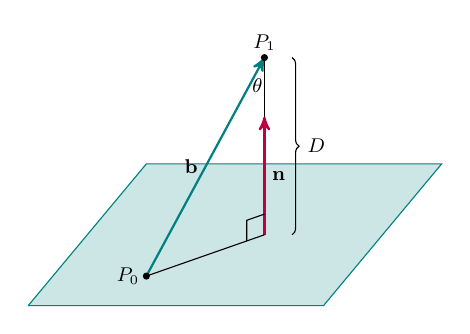
\begin{tikzpicture}[>=latex,xscale=.5*1.5, yscale=.5*1.5][font=\sf\small] 

\draw[teal, fill=teal!20, opacity=1] (0, 0)--++(5, 0)--++(2, 2.4)--++(-5, 0)--++(-2,-2.4);

\draw[purple, thick, ->, >=stealth'] ({4}, 1.2)--++(0, 2) node[black, right, pos=0.5, scale=0.8] {${\bf n}$};

\draw[samples=100, smooth, domain=4-2.0:4, variable=\x] 
		plot ({\x}, {1.2+0.7/2*(\x-4)}); 

\draw ({4-0.3}, {1.2+0.7/2*(4-0.3-4)}) --++(0, 0.35) -- ({4}, 1.55);

\draw[teal, thick, ->, >=stealth'] ({2.0}, {1.2+0.7/2*(2.0-4)}) -- (4, 4.2) node[black, left, pos=0.5, scale=0.8] {$\bf b$};

\draw (4, 3.2)--(4, 4.2);
\draw[fill] ({2.0}, {1.2+0.7/2*(2.0-4)}) circle(0.05) node[left, scale=0.8] {$P_0$};
\draw[fill]  (4, 4.2) circle(0.05) node[above, scale=0.8] {$P_1$};
\node[xshift=-2.5, yshift=-10, scale=0.8] at (4, 4.2) {$\theta$};

\draw [decoration={brace,raise=10, mirror},decorate] (4, 1.2)--++(0, 3)node[black, right, midway, pos=0.5, xshift=13, yshift=0, scale=0.8]{ $D$};

\end{tikzpicture}
\end{document}